% ------------------------------------------------------------
% LaTeX Template für die DHBW zum Schnellstart!
% Original: https://github.wdf.sap.corp/vtgermany/LaTeX-Template-DHBW
% ------------------------------------------------------------
% ---- Präambel mit Angaben zum Dokument
% LTeX: enabled=false

\documentclass[
	fontsize=12pt,           % Leitlinien sprechen von Schriftgröße 12.
	paper=A4,
	twoside=false,
	listof=totoc,            % Tabellen- und Abbildungsverzeichnis ins Inhaltsverzeichnis
	bibliography=totoc,      % Literaturverzeichnis ins Inhaltsverzeichnis aufnehmen
	titlepage,               % Titlepage-Umgebung anstatt \maketitle
	headsepline,             % horizontale Linie unter Kolumnentitel
	abstract,              % Überschrift einschalten, Abstract muss in {abstract}-Umgebung stehen
]{scrreprt}                  % Verwendung von KOMA-Report
\usepackage[utf8]{inputenc}  % UTF8 Encoding einschalten
\usepackage[ngerman,american]{babel}  % Neue deutsche Rechtschreibung
% \usepackage[T1]{fontenc}     % Ausgabe von westeuropäischen Zeichen (auch Umlaute)
% \usepackage{fontspec}
\usepackage{microtype}       % Trennung von Wörtern wird besser umgesetzt
\usepackage{lmodern}         % Nicht-gerasterte Schriftarten (bei MikTeX erforderlich)
\usepackage{graphicx}        % Einbinden von Grafiken erlauben
\usepackage{rotating}        % Rotieren von Grafiken ermöglichen
\usepackage{adjustbox}
\usepackage{wrapfig}         % Grafiken fließend im Text
\usepackage{setspace}        % Zeilenabstand \singlespacing, \onehalfspaceing, \doublespacing
\usepackage[
	%showframe,                % Ränder anzeigen lassen
	left=2.7cm, right=2.5cm,
	top=2.5cm,  bottom=2.5cm,
	includeheadfoot,
	a4paper
]{geometry}                      % Seitenlayout einstellen
\usepackage{scrlayer-scrpage}    % Gestaltung von Fuß- und Kopfzeilen
\usepackage[printonlyused]{acronym}             % Abkürzungen, Abkürzungsverzeichnis
\usepackage{titletoc}            % Anpassungen am Inhaltsverzeichnis
\contentsmargin{0.75cm}          % Abstand im Inhaltsverzeichnis zw. Punkt und Seitenzahl
\usepackage[                     % Klickbare Links (enth. auch "nameref", "url" Package)
  hidelinks,                     % Blende die "URL Boxen" aus.
  breaklinks=true                % Breche zu lange URLs am Zeilenende um
]{hyperref}
\usepackage[hypcap=true]{caption}% Anker Anpassung für Referenzen
\urlstyle{same}                  % Aktuelle Schrift auch für URLs
% Anpassung von autoref für Gleichungen (ergänzt runde Klammern) und Algorithm.
% Anstatt "Listing" kann auch z.B. "Code-Ausschnitt" verwendet werden. Dies sollte
% jedoch synchron gehalten werden mit \lstlistingname (siehe weiter unten).
\addto\extrasngerman{%
	\def\equationautorefname~#1\null{Gleichung~(#1)\null}
	\def\lstnumberautorefname{Zeile}
	\def\lstlistingautorefname{Listing}
	\def\algorithmautorefname{Algorithmus}
	% Damit einheitlich "Abschnitt 1.2[.3]" verwendet wird und nicht "Unterabschnitt 1.2.3"
	% \def\subsectionautorefname{Abschnitt}
}

% ---- Abstand verkleinern von der Überschrift 
\renewcommand*{\chapterheadstartvskip}{\vspace*{.5\baselineskip}}

% Hierdurch werden Schusterjungen und Hurenkinder vermieden, d.h. einzelne Wörter
% auf der nächsten Seite oder in einer einzigen Zeile.
% LaTeX kann diese dennoch erzeugen, falls das Layout ansonsten nicht umsetzbar ist.
% Diese Werte sind aber gute Startwerte.
\widowpenalty10000
\clubpenalty10000

% ---- Für das Quellenverzeichnis
\usepackage[
	backend = biber,                % Verweis auf biber
	language = auto,
	style = numeric,                % Nummerierung der Quellen mit Zahlen
	sorting = none,                 % none = Sortierung nach der Erscheinung im Dokument
	sortcites = true,               % Sortiert die Quellen innerhalb eines cite-Befehls
	block = space,                  % Extra Leerzeichen zwischen Blocks
	hyperref = true,                % Links sind klickbar auch in der Quelle
	%backref = true,                % Referenz, auf den Text an die zitierte Stelle
	bibencoding = auto,
	giveninits = true,              % Vornamen werden abgekürzt
	doi=false,                      % DOI nicht anzeigen
	isbn=false,                     % ISBN nicht anzeigen
    alldates=short                  % Datum immer als DD.MM.YYYY anzeigen
]{biblatex}
\addbibresource{library.bib}
\setcounter{biburlnumpenalty}{3000}     % Umbruchgrenze für Zahlen
\setcounter{biburlucpenalty}{6000}      % Umbruchgrenze für Großbuchstaben
\setcounter{biburllcpenalty}{9000}      % Umbruchgrenze für Kleinbuchstaben
\DeclareNameAlias{default}{family-given}  % Nachname vor dem Vornamen
\AtBeginBibliography{\renewcommand{\multinamedelim}{\addslash\space
}\renewcommand{\finalnamedelim}{\multinamedelim}}  % Schrägstrich zwischen den Autorennamen
\DefineBibliographyStrings{german}{
  urlseen = {Einsichtnahme:},                      % Ändern des Titels von "besucht am"
}
\usepackage[babel,german=quotes]{csquotes}         % Deutsche Anführungszeichen + Zitate


% ---- Für Mathevorlage
\usepackage{amsmath}    % Erweiterung vom Mathe-Satz
\usepackage{amssymb}    % Lädt amsfonts und weitere Symbole
\usepackage{MnSymbol}   % Für Symbole, die in amssymb nicht enthalten sind.

% ---- Für chemische Formeln
\usepackage{mhchem}

% ---- Für Quellcodevorlage
\usepackage{scrhack}                    % Hack zur Verw. von listings in KOMA-Script
\usepackage{listings}                   % Darstellung von Quellcode
\usepackage{xcolor}                     % Einfache Verwendung von Farben
% -- Eigene Farben für den Quellcode
\definecolor{JavaLila}{rgb}{0.4,0.1,0.4}
\definecolor{JavaGruen}{rgb}{0.3,0.5,0.4}
\definecolor{JavaBlau}{rgb}{0.0,0.0,1.0}
\definecolor{ABAPKeywordsBlue}{HTML}{6000ff}
\definecolor{ABAPCommentGrey}{HTML}{808080}
\definecolor{ABAPStringGreen}{HTML}{4da619}
\definecolor{PyKeywordsBlue}{HTML}{0000AC}
\definecolor{PyCommentGrey}{HTML}{808080}
\definecolor{PyStringGreen}{HTML}{008080}
% -- Farben für ABAP CDS
\definecolor{CDSString}{HTML}{FF8C00}
\definecolor{CDSKeywords}{HTML}{6000ff}
\definecolor{CDSAnnotation}{HTML}{00BFFF}
\definecolor{CDSComment}{HTML}{808080}
\definecolor{CDSFunc}{HTML}{FF0000}

% -- Default Listing-Styles

\lstset{
	% Das Paket "listings" kann kein UTF-8. Deswegen werden hier 
	% die häufigsten Zeichen definiert (ä,ö,ü,...)
	literate=%
		{á}{{\'a}}1 {é}{{\'e}}1 {í}{{\'i}}1 {ó}{{\'o}}1 {ú}{{\'u}}1
		{Á}{{\'A}}1 {É}{{\'E}}1 {Í}{{\'I}}1 {Ó}{{\'O}}1 {Ú}{{\'U}}1
		{à}{{\`a}}1 {è}{{\`e}}1 {ì}{{\`i}}1 {ò}{{\`o}}1 {ù}{{\`u}}1
		{À}{{\`A}}1 {È}{{\'E}}1 {Ì}{{\`I}}1 {Ò}{{\`O}}1 {Ù}{{\`U}}1
		{ä}{{\"a}}1 {ë}{{\"e}}1 {ï}{{\"i}}1 {ö}{{\"o}}1 {ü}{{\"u}}1
		{Ä}{{\"A}}1 {Ë}{{\"E}}1 {Ï}{{\"I}}1 {Ö}{{\"O}}1 {Ü}{{\"U}}1
		{â}{{\^a}}1 {ê}{{\^e}}1 {î}{{\^i}}1 {ô}{{\^o}}1 {û}{{\^u}}1
		{Â}{{\^A}}1 {Ê}{{\^E}}1 {Î}{{\^I}}1 {Ô}{{\^O}}1 {Û}{{\^U}}1
		{œ}{{\oe}}1 {Œ}{{\OE}}1 {æ}{{\ae}}1 {Æ}{{\AE}}1 {ß}{{\ss}}1
		{ű}{{\H{u}}}1 {Ű}{{\H{U}}}1 {ő}{{\H{o}}}1 {Ő}{{\H{O}}}1
		{ç}{{\c c}}1 {Ç}{{\c C}}1 {ø}{{\o}}1 {å}{{\r a}}1 {Å}{{\r A}}1
		{€}{{\euro}}1 {£}{{\pounds}}1 {«}{{\guillemotleft}}1
		{»}{{\guillemotright}}1 {ñ}{{\~n}}1 {Ñ}{{\~N}}1 {¿}{{?`}}1,
	breaklines=true,        % Breche lange Zeilen um 
	breakatwhitespace=true, % Wenn möglich, bei Leerzeichen umbrechen
	% Symbol für Zeilenumbruch einfügen
	prebreak=\raisebox{0ex}[0ex][0ex]{\ensuremath{\rhookswarrow}},
	postbreak=\raisebox{0ex}[0ex][0ex]{\ensuremath{\rcurvearrowse\space}},
	tabsize=4,                                 % Setze die Breite eines Tabs
	basicstyle=\ttfamily\small,                % Grundsätzlicher Schriftstyle
	columns=fixed,                             % Besseres Schriftbild
	numbers=left,                              % Nummerierung der Zeilen
	%frame=single,                             % Umrandung des Codes
	showstringspaces=false,                    % Keine Leerzeichen hervorheben
	keywordstyle=\color{blue},
	ndkeywordstyle=\bfseries\color{darkgray},
	identifierstyle=\color{black},
	commentstyle=\itshape\color{JavaGruen},   % Kommentare in eigener Farbe
	stringstyle=\color{JavaBlau},             % Strings in eigener Farbe,
	captionpos=b,                             % Bild*unter*schrift
	xleftmargin=5.0ex
}

% ---- Eigener JAVA-Style für den Quellcode
\renewcommand{\ttdefault}{pcr}               % Schriftart, welche auch fett beinhaltet
\lstdefinestyle{EigenerJavaStyle}{
	language=Java,                             % Syntax Highlighting für Java
	%frame=single,                             % Umrandung des Codes
	keywordstyle=\bfseries\color{JavaLila},    % Keywords in eigener Farbe und fett
	commentstyle=\itshape\color{JavaGruen},    % Kommentare in eigener Farbe und italic
	stringstyle=\color{JavaBlau}               % Strings in eigener Farbe
}

% ---- Eigener ABAP-Style für den Quellcode
\renewcommand{\ttdefault}{pcr}
\lstdefinestyle{EigenerABAPStyle}{
	language=[R/3 6.10]ABAP,
	morestring=[b]\|,                          % Für Pipe-Strings
	morestring=[b]\`,                          % für Backtick-Strings
	keywordstyle=\bfseries\color{ABAPKeywordsBlue},
	commentstyle=\itshape\color{ABAPCommentGrey},
	stringstyle=\color{ABAPStringGreen},
	tabsize=2,
	morekeywords={
		types,
		@data,
		as,
		lower,
		start,
		selection,
		order,
		by,
		inner,
		join,
		key,
		end,
		cast
	}
}

% ---- Eigener Python-Style für den Quellcode
\renewcommand{\ttdefault}{pcr}
\lstdefinestyle{EigenerPythonStyle}{
	language=Python,
	columns=flexible,
	keywordstyle=\bfseries\color{PyKeywordsBlue},
	commentstyle=\itshape\color{PyCommentGrey},
	stringstyle=\color{PyStringGreen}
}

%----- ABAP-CDS-View language
\lstdefinelanguage{ABAPCDS}{
	sensitive=false,
	%Keywords
	morekeywords={define,
		view,
		as,
		select,
		from,
		inner,
		join,
		on,
		key,
		case,
		when,
		then,
		else,
		end,
		true,
		false,
		cast,
		where,
		and,
		distinct,
		group,
		by,
		having,
		min,
		sum,
		max,
		count,
		avg
	},
	%Methoden
	morekeywords=[2]{
		div,
		currency\_conversion,
		dats\_days\_between,
		concat\_with\_space,
		dats\_add_days,
		dats\_is\_valid,
		dats\_add\_months,
		unit\_conversion,
		division,
		mod,
		abs,
		floor,
		ceil,
		round,
		concat,
		replace,
		substring,
		left,
		right,
		length
	},
	morecomment=[s][\color{CDSAnnotation}]{@}{:},
	morecomment=[l][\itshape\color{CDSComment}]{//},
	morecomment=[s][\itshape\color{CDSComment}]{/*}{*/},
	morestring=[b][\color{CDSString}]',
	keywordstyle=\bfseries\color{CDSKeywords},
	keywordstyle=[2]\color{CDSFunc}
}

  % Weitere Details sind ausgelagert

\usepackage{algorithm}                  % Für Algorithmen-Umgebung (ähnlich wie lstlistings Umgebung)
\usepackage{algpseudocode}              % Für Pseudocode. Füge "[noend]" hinzu, wenn du kein "endif",
                                        % etc. haben willst.

\makeatletter                           % Sorgt dafür, dass man @ in Namen verwenden kann.
                                        % Ansonsten gibt es in der nächsten Zeile einen Compilefehler.
\renewcommand{\ALG@name}{Algorithmus}   % Umbenennen von "Algorithm" im Header der Listings.
\makeatother                            % Zeichen wieder zurücksetzen
\renewcommand{\lstlistingname}{Listing} % Erlaubt das Umbenennen von "Listing" in anderen Titel.

% ---- Tabellen
\usepackage{booktabs}  % Für schönere Tabellen. Enthält neue Befehle wie \midrule
\usepackage{multirow}  % Mehrzeilige Tabellen
\usepackage{siunitx}   % Für SI Einheiten und das Ausrichten Nachkommastellen
\sisetup{locale=DE, range-phrase={~bis~}, output-decimal-marker={,}} % Damit ein Komma und kein Punkt verwendet wird.
\usepackage{xfrac} % Für siunitx Option "fraction-function=\sfrac"

% ---- Für Definitionsboxen in der Einleitung
\usepackage{amsthm}                     % Liefert die Grundlagen für Theoreme
\usepackage[framemethod=tikz]{mdframed} % Boxen für die Umrandung
% ---- Definition für Highlight Boxen

% ---- Grundsätzliche Definition zum Style
\newtheoremstyle{defi}
  {\topsep}         % Abstand oben
  {\topsep}         % Abstand unten
  {\normalfont}     % Schrift des Bodys
  {0pt}             % Einschub der ersten Zeile
  {\bfseries}       % Darstellung von der Schrift in der Überschrift
  {:}               % Trennzeichen zwischen Überschrift und Body
  {.5em}            % Abstand nach dem Trennzeichen zum Body Text
  {\thmname{#3}}    % Name in eckigen Klammern
\theoremstyle{defi}

% ------ Definition zum Strich vor eines Texts
\newmdtheoremenv[
  hidealllines = true,       % Rahmen komplett ausblenden
  leftline = true,           % Linie links einschalten
  innertopmargin = 0pt,      % Abstand oben
  innerbottommargin = 4pt,   % Abstand unten
  innerrightmargin = 0pt,    % Abstand rechts
  linewidth = 3pt,           % Linienbreite
  linecolor = gray!40,       % Linienfarbe
]{defStrich}{Definition}     % Name der des formats "defStrich"

% ------ Definition zum Eck-Kasten um einen Text
\newmdtheoremenv[
  hidealllines = true,
  innertopmargin = 6pt,
  linecolor = gray!40,
  singleextra={              % Eck-Markierungen für die Definition
    \draw[line width=3pt,gray!50,line cap=rect] (O|-P) -- +(1cm,0pt);
    \draw[line width=3pt,gray!50,line cap=rect] (O|-P) -- +(0pt,-1cm);
    \draw[line width=3pt,gray!50,line cap=rect] (O-|P) -- +(-1cm,0pt);
    \draw[line width=3pt,gray!50,line cap=rect] (O-|P) -- +(0pt,1cm);
  }
]{defEckKasten}{Definition}  % Name der des formats "defEckKasten"  % Weitere Details sind ausgelagert

% ---- Für Todo Notes
\usepackage{todonotes}
\setlength {\marginparwidth }{2cm}      % Abstand für Todo Notizen

\lstdefinelanguage{JavaScript}{
  morekeywords=[1]{break, case, catch, continue, debugger, default, delete, do, else, finally, for, function, if, in, instanceof, new, return, switch, this, throw, try, typeof, var, void, while, with, require, then, const},
  morecomment=[l]{//},
  morecomment=[s]{/*}{*/},
  morestring=[b]{'},
  morestring=[b]{"},
  morestring=[b]{`},
%   alsoletter={\\'},
  stringstyle=\color[rgb]{0.3,0.5,0.4},
  sensitive=true
}

\lstdefinelanguage{Docker}{
	% Keywords as defined in the language grammar
	morekeywords=[1]{%
	  FROM,RUN,COPY,WORKDIR,LABEL,USER,ENTRYPOINT,EXPOSE,CMD},
	% Built-in functions
	morekeywords=[2]{},
	% Pre-declared types
	morekeywords=[3]{},
	% Constants and zero value
	morekeywords=[4]{},
	% Strings : "foo", 'bar', `baz`
	morestring=[b]{"},
	morestring=[b]{'},
	morestring=[b]{`},
	% Comments : /* cpmment */ and // comment
	comment=[l]{\#},
	morecomment=[s]{/*}{*/},
	stringstyle=\color[rgb]{0.3,0.5,0.4},
	% Options
	sensitive=true
}

\lstdefinelanguage{Golang}%
  {morekeywords=[1]{package,import,func,type,struct,return,defer,panic,%
     recover,select,var,const,iota,},%
   morekeywords=[2]{string,uint,uint8,uint16,uint32,uint64,int,int8,int16,%
     int32,int64,bool,float32,float64,complex64,complex128,byte,rune,uintptr,%
     error,interface},%
   morekeywords=[3]{map,slice,make,new,nil,len,cap,copy,close,true,false,%
     delete,append,real,imag,complex,chan,},%
   morekeywords=[4]{for,break,continue,range,go,goto,switch,case,fallthrough,if,%
     else,default,},%
   morekeywords=[5]{Println,Printf,Error,Print,},%
   sensitive=true,%
   morecomment=[l]{//},%
   morecomment=[s]{/*}{*/},%
   morestring=[b]',%
   morestring=[b]",%
   morestring=[s]{`}{`},%
   tabsize = 2,%
}

\usepackage{xurl}

% ---- Elektronische Version oder Gedruckte Version?
% ---- Unterschied: Die elektronische Version enthält keinen Platzhalter für die Unterschrift
\usepackage{ifthen}
\newboolean{e-Abgabe}
\setboolean{e-Abgabe}{false}    % false=gedruckte Fassung

% ---- Persönlichen Daten:
\newcommand{\titel}{Redesigning and Implementing the Bootstrap of Large Scale Kubernetes Enterprise Infrastructure through Automated Self Contained CLI}
\newcommand{\titelheader}{Bootstrapping Kubernetes Infrastructure} % TOOD: is this even needed?
\newcommand{\arbeit}{Project 2b (T3\_2000)}
\newcommand{\studiengang}{Computer Science (Informatik)}
\newcommand{\studienjahr}{2020}
\newcommand{\autor}{Yannik Schiebelhut}
\newcommand{\autorReverse}{Schiebelhut, Yannik}
\newcommand{\verfassungsort}{Karlsruhe}
\newcommand{\matrikelnr}{3354235}
\newcommand{\kurs}{TINF20B1}
\newcommand{\bearbeitungsmonat}{September 2022}
\newcommand{\abgabe}{September 19, 2022}
\newcommand{\bearbeitungszeitraum}{July 4, 2022 - September 19, 2022}
\newcommand{\firmaName}{SAP SE}
\newcommand{\firmaStrasse}{Dietmar-Hopp-Allee 16}
\newcommand{\firmaPlz}{69190 Walldorf, Deutschland}
\newcommand{\betreuerFirma}{Samed Guener} % TODO: doch Jan einsetzen? TODO: Mit Umlaut?
\newcommand{\betreuerDhbw}{Prof. Dr. Johannes Freudenmann}

% ---- Metainformation für das PDF Dokument
\hypersetup{
	pdftitle    = {\titel},
	pdfsubject  = {\arbeit},
	pdfauthor   = {\autor},
	%pdfkeywords = {Keywords angeben},
	pdfcreator  = {LaTeX},
	%pdfproducer = {in der Regel pdfTeX}
}

% ---- Definition der Kopf- und Fußzeilen
\clearscrheadfoot                               % Löschen von LaTeX Standard
\automark[section]{chapter}                     % Füllen von section und chapter
\renewcommand*{\chaptermarkformat}{}            % Entfernt die Kapitelnummer
\renewcommand*{\sectionmarkformat}{}            % Entfernt die Sectionnummer
% Angaben [für "plain"]{für "scrheadings"}
% \ihead[]{\titelheader}                          % Kopfzeile links
\ihead{\ifthenelse{\value{chapter}>0}{\chaptername~\thechapter}{}}
\chead[]{}                                      % Kopfzeile mitte
% \ohead[]{\rightmark}                            % Kopfzeile rechts
\ohead{\ifthenelse{\value{chapter}>0}{\headmark}{}}
\ifoot[]{}                                      % Fußzeile links
\cfoot*{\sffamily\pagemark}                     % Fußzeile mitte
\ofoot[]{}                                      % Fußzeile rechts
\KOMAoptions{
   headsepline = 0.2pt,                         % Liniendicke Kopfzeile
   footsepline = false                          % Liniendicke Fußzeile
}

% ---- Hilfreiches
\newcommand{\zB}{z.\,B. }   % "z.B." mit kleinem Leeraum dazwischen (ohne wäre nicht korrekt)
\newcommand{\dash}{d.\,h. }
\newcommand{\Dash}{D.\,h. }

\newcommand{\code}[1]{\texttt{#1}} % Ist einfacher zu schreiben als ständig \texttt und erlaubt
                                   % Änderungen im Nachhinein, wenn man z.B. Inline-Code anders stylen möchte.

% ---- Silbentrennung (falls LaTeX defaults falsch / nicht gewünscht sind)
\hyphenation{HANA}         % anstatt HA-NA
\hyphenation{Graph-Script} % anstatt GraphS-cript

% ---- Beginn des Dokuments
\begin{document}
\setlength{\parindent}{0pt}              % Keine Paragraphen Einrückung.
                                         % Dafür haben wir den Abstand zwischen den Paragraphen.
\setcounter{secnumdepth}{2}              % Nummerierungstiefe fürs Inhaltsverzeichnis
\setcounter{tocdepth}{1}                 % Tiefe des Inhaltsverzeichnisses. Ggf. so anpassen,
                                         % dass das Verzeichnis auf eine Seite passt.
\sffamily                                % Serifenlose Schrift verwenden.

% ---- Vorspann
% ------ Titelseite
\singlespacing
\begin{otherlanguage}{ngerman}
    \thispagestyle{empty}
\begin{titlepage}
\enlargethispage{4cm}

\begin{figure}           % Logo vom Ausbildungsbetrieb und der DHBW
	% \vspace*{-5mm} % Sollte dein Titel zu lang werden, kannst du mit diesem "Hack" 
	%                  den Inhalt der Seite nach oben schieben.
	\begin{minipage}{0.49\textwidth}
		\flushleft
		
\includegraphics[height=2.5cm]{Bilder/Logos/Logo_SAP.pdf} 
	\end{minipage}
	\hfill
	\begin{minipage}{0.49\textwidth}
		\flushright
		
\includegraphics[height=2.5cm]{Bilder/Logos/Logo_DHBW.pdf} 
	\end{minipage}
\end{figure} 
\vspace*{0.1cm}

\begin{center}
	\huge{\textbf{\titel}}\\[1.5cm]
	\Large{\textbf{\arbeit}}\\[0.5cm]
	\normalsize{in the context of the examination for the\\[1ex] \textbf{Bachelor of Science (B.Sc.)}}\\[0.5cm]
	\Large{in \studiengang}\\[1ex]
	\normalsize{at the Cooperative State University Baden-Württemberg Karlsruhe}\\[1cm]
	\normalsize{by}\\[1ex] \Large{\textbf{\autor}} \\[1cm]
\end{center}

\begin{center}
	\vfill
	\begin{tabular}{ll}
		Submission Date:                               & \abgabe \\[0.2cm]
		Processing period:                             & \bearbeitungszeitraum \\[0.2cm]
		Matriculation number, Course:                  & \matrikelnr , \kurs \\[0.2cm]
		Training institution:                          & \firmaName \\
		                                               & \firmaStrasse \\
		                                               & \firmaPlz \\[0.2cm]
		Supervisor of the training institution:        & \betreuerFirma \\[0.2cm]
		Appraiser of the Cooperative State University: & \betreuerDhbw \\[2cm]
	\end{tabular} 
\end{center}
\end{titlepage}
  % Titelseite
\end{otherlanguage}
\newcounter{savepage}
\pagenumbering{Roman}                    % Römische Seitenzahlen
\onehalfspacing

\begin{otherlanguage}{ngerman}
    % ------ Erklärung, Sperrvermerk, Abstact
    \chapter*{Eidesstattliche Erklärung}
Ich versichere hiermit, dass ich meine \arbeit{} mit dem Thema:
\begin{quote}
	\textit{\titel}
\end{quote} 
gemäß § 5 der \enquote{Studien- und Prüfungsordnung DHBW Technik} vom 29. September 2017 selbstständig verfasst und keine anderen als die angegebenen Quellen und Hilfsmittel benutzt habe. Die Arbeit wurde bisher keiner anderen Prüfungsbehörde vorgelegt und auch nicht veröffentlicht.

\vspace{0.25cm}

Ich versichere zudem, dass die eingereichte elektronische Fassung mit der gedruckten Fassung übereinstimmt.

\vspace{1cm}

\verfassungsort, den \today \\[0.5cm]
\ifthenelse{\boolean{e-Abgabe}}
	{\underline{Gez. \autor}}
	{\makebox[6cm]{\hrulefill}}\\ 
\autorReverse

    \chapter*{Sperrvermerk}
Die nachfolgende Arbeit enthält vertrauliche Daten der:
\begin{quote}
	\firmaName \\
	\firmaStrasse \\
	\firmaPlz
\end{quote}

\vspace{0.5cm}

Der Inhalt dieser Arbeit darf weder als Ganzes noch in Auszügen Personen außerhalb des Prüfungsprozesses und des Evaluationsverfahrens zugänglich gemacht werden, sofern keine anderslautende Genehmigung vom Dualen Partner vorliegt.

    \renewcommand{\abstractname}{Abstract} % Veränderter Name für das Abstract
\begin{abstract}
\begin{addmargin}[1.5cm]{1.5cm}        % Erhöhte Ränder, für Abstract Look
\thispagestyle{plain}                  % Seitenzahl auf der Abstract Seite

\begin{center}
\small\textit{- Deutsch -}             % Angabe der Sprache für das Abstract
\end{center}

\vspace{0.25cm}

% LTeX: language=de-DE

Platzhalter

\end{addmargin}
\end{abstract}
    \renewcommand{\abstractname}{Abstract} % Veränderter Name für das Abstract
\begin{abstract}
\begin{addmargin}[1.5cm]{1.5cm}        % Erhöhte Ränder, für Abstract Look
\thispagestyle{plain}                  % Seitenzahl auf der Abstract Seite

\begin{center}
\small\textit{- English -}             % Angabe der Sprache für das Abstract
\end{center}

\vspace{0.25cm}

% LTeX: language=en-US

In order to raise cross company processes to a new level SAP is working on the development of \acl*{ccwf}.
The shared process data is to be imported into \emph{Signavio Process Intelligence} to be analyzed with process mining and to be presented in \aclp*{kpi}.
Since \acl*{ccwf} uses the \emph{SAP Blockchain} to store data the preparation of the data for analysis within Signavio is a challenge.

\vspace{0.25cm}

In the context of this report, these difficulties will first be discussed.
It then deals with the conceptual design of a data integration process.
For this purpose, on the one hand, it is discussed where the conversion of the data from \acl*{ccwf} into the target format should be carried out.
On the other hand, different transport routes are discussed, through which the processed data should be made available in Signavio Process Intelligence.
Based on the developed concept, a prototype of the data integration is implemented.

\end{addmargin}
\end{abstract}
\end{otherlanguage}

% ------ Inhaltsverzeichnis
\singlespacing
\tableofcontents

% ------ Verzeichnisse
\renewcommand*{\chapterpagestyle}{plain}
\pagestyle{plain}
% \chapter*{Formelverzeichnis}
\addcontentsline{toc}{chapter}{Formelverzeichnis} % Hinzufügen zum Inhaltsverzeichnis 

% Definition des neuen Befehls für das Einfügen der Abkürzung der Einheit
\newcommand{\acrounit}[1]{
  \acroextra{\makebox[18mm][l]{\si[per-mode=fraction,fraction-function=\sfrac]{#1}}}
}
\begin{acronym}[dmin] % längstes Kürzel wird verw. für den Abstand zw. Kürzel u. Text

	% Alphabetisch selbst sortieren - nicht verwendete Formeln rausnehmen!
	% Allgemein: \acro{KÜRZEL}[ABKÜRZUNG]{\acrounit{SI-EINHEIT}BESCHREIBUNG}

	\acro{A}[\ensuremath{A}]{\acrounit{mm^2}Fläche}	
	\acro{D}[\ensuremath{D}]{\acrounit{mm}Werkstückdurchmesser}	
	\acro{dmin}[\ensuremath{d\textsubscript{min}}]{\acrounit{mm}kleinster Schaftdurchmesser}	
	\acro{L1}[\ensuremath{L\textsubscript{1}}]{\acrounit{mm}Länge des Werkstückes Nr. 1}	
	\acro{Fwinkel}[]{\acrounit{Grad}Freiwinkel}	
	\acro{Kwinkel}[]{\acrounit{Grad}Keilwinkel}

\end{acronym}

\chapter*{List of Abbreviations}
\addcontentsline{toc}{chapter}{List of Abbreviations} % Hinzufügen zum Inhaltsverzeichnis 

\begin{acronym}[BPMN] % längstes Kürzel wird verw. für den Abstand zw. Kürzel u. Text

	% Alphabetisch selbst sortieren - nicht verwendete Kürzel rausnehmen!
	\acro{acl}[ACL]{Access Control List}
	% \acro{AIR}{Adobe Integrated Runtime}
	% \acro{AJAX}{Asynchronous Javascript and XML}
	% \acro{ANSI}{American National Standards Institute}
	\acro{api}[API]{Application Programming Interface}
	% \acro{AR}{Augmented Reality}
	\acro{aws}[AWS]{Amazon Web Services}
	% \acro{BAPI}{Business Application Programming Interface}
	% \acro{BIOS}{Basic Input Output System}
	\acro{bpmn}[BPMN]{Business Process Model and Notation}
	\acro{ccwf}[ccWF]{Cross-Company Workflow}
	% \acro{CDMA}{Code Division Multiple Access}
	\acro{cicd}[CICD]{Continuous Integration and Continuous Delivery}
	\acro{cli}[CLI]{command-line interface}
	\acro{csv}[CSV]{Comma-Separated Values}
	\acro{eks}[EKS]{Elastic Kubernetes Service}
	\acro{erp}[ERP]{Enterprise Resource Planning}
	\acro{hcl}[HCL]{HashiCorp Configuration Language}
	\acro{hs2}[HS2]{High Speed 2}
	\acro{http}[HTTP]{Hypertext Transfer Protocol}
	% \acro{HTTPS}{Hypertext Transfer Protocol Secure}
	\acro{iaas}[IaaS]{Infrastructure as a Service}
	\acro{iac}[IaC]{Infrastructure as Code}
	% \acro{IP}{Internet Protocol}
	% \acro{ISBN}{Internationale Standardbuchnummer}
	% \acrodefplural{ISBN}[ISBNs]{Internationale Standardbuchnummern}
	\acro{json}[JSON]{JavaScript Object Notation}
	\acro{kpi}[KPI]{Key Performance Indicator}
	% \acro{OData}{Open Data Protocol}
	\acro{rest}[REST]{Representational State Transfer}
	\acro{s3}[S3]{Simple Storage Service}
	\acro{saml}[SAML]{Security Assertion Markup Language}
	\acro{sdk}[SDK]{Software Development Kit}
	% \acro{SEO}{Search Engine Optimization}
	\acro{sql}[SQL]{Structured Query Language}
	% \acro{SSH}{Secure Shell}
	% \acro{UEFI}{Unified Extensible Firmware Interface}
	% \acro{URI}{Uniform Resource Identifier}
	\acro{url}[URL]{Uniform Resource Locator}
	% \acro{USB}{Universal Serial Bus}
	\acro{vcs}[VCS]{Version Control System}
	% \acro{VLAN}{Virtual Local Area Network}
	% \acro{WYSISWG}{What You See Is What You Get}
	\acro{xes}[XES]{eXtensible Event Stream}
	% \acro{XSL}{Extensible Stylesheet Language}

\end{acronym}
\listoffigures                          % Erzeugen des Abbildungsverzeichnisses 
% \listoftables                           % Erzeugen des Tabellenverzeichnisses
\renewcommand{\lstlistlistingname}{List of Code Listings}
\lstlistoflistings                      % Erzeugen des Listenverzeichnisses
\setcounter{savepage}{\value{page}}


% ---- Inhalt der Arbeit
\cleardoublepage
\pagenumbering{arabic}                  % Arabische Seitenzahlen für den Hauptteil
\setlength{\parskip}{0.5\baselineskip}  % Abstand zwischen Absätzen
\rmfamily
\renewcommand*{\chapterpagestyle}{scrheadings}
\pagestyle{scrheadings}
\onehalfspacing
% \include{content goes here}
\chapter{Introduction}
\section{Motivation}
Modern enterprise infrastructure for software development often makes use of cloud computing to dynamically adapt infrastructure to the fast-paced world of agile development.
The setup process of one so-called cluster is traditionally done by hand and can easily require multiple days of work to complete.
Obviously, in consequence of the required man-hours, this manual deployment is rather costly and time-consuming.
Also, humans are prune to error.
In a manual task that big, it is very likely for unforeseeable errors to occur.
Finding these mistakes can eventually take additional time.

As a conclusion, it is desired to automate as much of a clusters' deployment process as possible.
There are already various tools available that can be leveraged to perform an automated deployment of a declared cluster infrastructure.
But even these automatization tools require some perquisites to run, like a technical access user with access to the necessary resources and access keys to make use of this user, which still have to be created manually or with the help of bare-bones scripts.
The process of fulfilling these requirements is referred to as bootstrap.

\section{Goal}
Goal of this project is to simplify the bootstrap of a cluster by integrating the necessary functionality into a \ac{cli} which is currently developed by the supervising department.
Also, the usage should be convenient and, beside providing login data for the cloud provider and credential store, minimal user input should be required to perform the bootstrap.
Furthermore, the newly developed \ac{cli} is required to be able to get executed by an automated build server.
The ways of user interaction have to be designed accordingly.

\section{Approach}

\chapter{Fundamentals}
\section{Go}
Go (also known as Golang) is an open source programming language that was started at Google in 2007 and initially launched in 2009.
The language was designed to face engineering challenges at Google with the goal to make it \enquote{easy to build simple, reliable and efficient software}. \cite{pike.2020, golang.github}
By now, the compiled and statically typed language \cite{chris.2021} is widely used, and the way it approaches network concurrency and software engineering has influenced other languages to a noticeable extent. \cite{pike.2020}
Through its structure Go supports programming on various levels of abstraction.
For instance, one can embed Assembler or C code into a Go program or on the other hand combine groups of components into bigger, more complex components to realize abstract design patterns. \cite{Maurer2021}
Nowadays, Go is a popular choice for everything related to DevOps and therefore also for the development of command line tools. \cite{mike.2020}

Go also tries to provide its own, official solutions for common tasks in software development.
When installing Go, it comes packed alongside with a formatter (which shall ensure uniform styling across all programs written in Go) and an included suite for unit testing, just to name a few examples.
Furthermore, Go supports generating documentation based on comments in the source code; much alike JavaDoc.
Go features an extensive standard library which depicts a good starting point for developing your own applications.
In case one wants to include a third party library, this can be done via the \emph{go get} command.
It fetches the necessary resources (usually directly from a \ac{vcs}) and saves the modules as a dependency in the \emph{go.mod} file. \cite{go.tour, go.docs}

% \begin{itemize}
%     \item toolchain (uniform formatter, included test suite, source code based generation of documentation)
%     \item third party modules repo / go get
%     \item extensive standard library
%     \item (cite from golang.org tutorial)
% \end{itemize}

% started in 2007 released in 2009
% open source, compiled, and statically typed programming language (https://www.freecodecamp.org/news/what-is-go-programming-language/)
% face engineering challenges at Google (https://go.dev/solutions/google/)
% goals: make it "easy to build simple, reliable and efficient software" (https://github.com/golang/go)
% by now widely used
% network concurrency and software engineering are influencing other languages (https://go.dev/solutions/google/)
% through its structure go supports programming on various layers of abstraction (cite from book here)
%     supports embedded assembler and c
%     suitable for realizing abstract design patterns

\subsection{Cobra}
Cobra is an open source library for Go.
Its aim is to provide developers with an easy way to create modern \ac{cli} applications.
The cobra library is being used by noticeable projects like the \ac{cli}s for Kubernetes or for GitHub.
The idea behind Cobra's intended command schema is that commands of a well constructed \ac{cli} should read like sentences.
This way, new users that are familiar with \acp{cli} in general quickly feel native because interacting with the \ac{cli} feels more natural.
In this approach, a command represents a certain action that the \ac{cli} can perform.
This action than take arguments and flags to further specify on which objects and in which way the command should take action.
With Cobra, one can also easily create nested subcommands.
This means that a before mentioned command can also be divided into multiple sub-actions to enable detailed handling of complex actions.
Further, benefits of Cobra are, among others, the automated generation of autocompletion for the most common shells as well as the ability to automatically create man pages. \cite{cobra.github, cobra.dev}
The \ac{cli} that the supervising department is currently developing is build upon Cobra.


% \begin{itemize}
% 	\item open source library
%     \item modern cli applications
%     \item "namenhafte" projects like Kubernetes, GitHub CLI
%     \item subcommand-based -> explain
%     \item nested subcommands
%     \item can automatically generate autocomplete
%     \item helps in generating man pages \cite{cobra.github}
% \end{itemize}

\section{Kubernetes}
\label{sec:kubernetes}
Kubernetes (often short: k8s) is an open source solution to ease up and automate management of container based services.
It follows a declarative paradigm.
This means that the user just needs to describe the desired state -- for example through the use of configuration files or via the Kubernetes \ac{cli} -- and Kubernetes determines the steps by itself which are necessary to reach and maintain this state.
Kubernetes also enables users to dynamically scale their applications and services.
This means that the amount of resources, that are dedicated to an application, is adapted during runtime dependent, for example, on the current number of users.
Furthermore, Kubernetes can perform load balancing and redundancy between different instances of the same service.
\cite{Bloß2019, wasistk8s}

One instance of a Kubernetes system is called a cluster.
A Cluster is composed of multiple nodes (which usually are virtual machines or physical servers) which run the actual applications.
An Application runs inside some kind of container, internally called Pod.
The interaction with a cluster is managed by the so-called \emph{Kubernetes Master}.
It is a central controlling unit.
The user actually never interacts with the nodes themselves directly.
\cite{k8skonzepte}

\section{Gardener}
Even though there are tools that help with creating and updating single Kubernetes clusters, it is rather hard to manage many clusters.
This is where Gardener comes into play.
It is a Kubernetes native extension that manages Kubernetes clusters as a service, packing the performance to manage up to thousands of clusters.
One key concept that is applied is so-called self-hosting.
This means that Kubernetes components are run inside of Kubernetes clusters, and is done because Kubernetes is the go-to way to easily manage software in the cloud. \cite{gardener.architecture, gardener.blog1, gardener.blog2, gardener.cloud}

Gardener's architecture is constructed much like Kubernetes itself although not individual Pods are managed but entire clusters.
The root of all is the so-called \emph{Garden Cluster}.
It is the main interface for the Gardener administrator and hosts, among others, the Garden Cluster control plane, the Gardener dashboard, the Gardener \ac{api} server, the Gardener controller manager, and the Gardener scheduler.
Then there are two other types of clusters, \emph{Seed Clusters} and \emph{Shoot Clusters}.
One Seed Clusters manages the control planes (thus \ac{api} server, scheduler, controller manager, machine controller etc.) of its Shoot Clusters.
There is at least one Seed Cluster per \ac{iaas} provider and region.
The Shoot Clusters control planes are deployed as Pods inside the Seed Cluster, can therefore be created with standard Kubernetes deployment and support rolling updates.
Shoot Clusters only contain worker nodes and are the Kubernetes Clusters that actually become available to the end-user and can be ordered in a declarative way.
The clusters created by Gardener are vanilla Kubernetes clusters independent of the underlying cloud provider. \cite{gardener.blog2, wasistgardener}
(More details of the described architecture can be seen in \autoref{fig:gardener-architecture}.)

\begin{figure}[H]
    \centering
    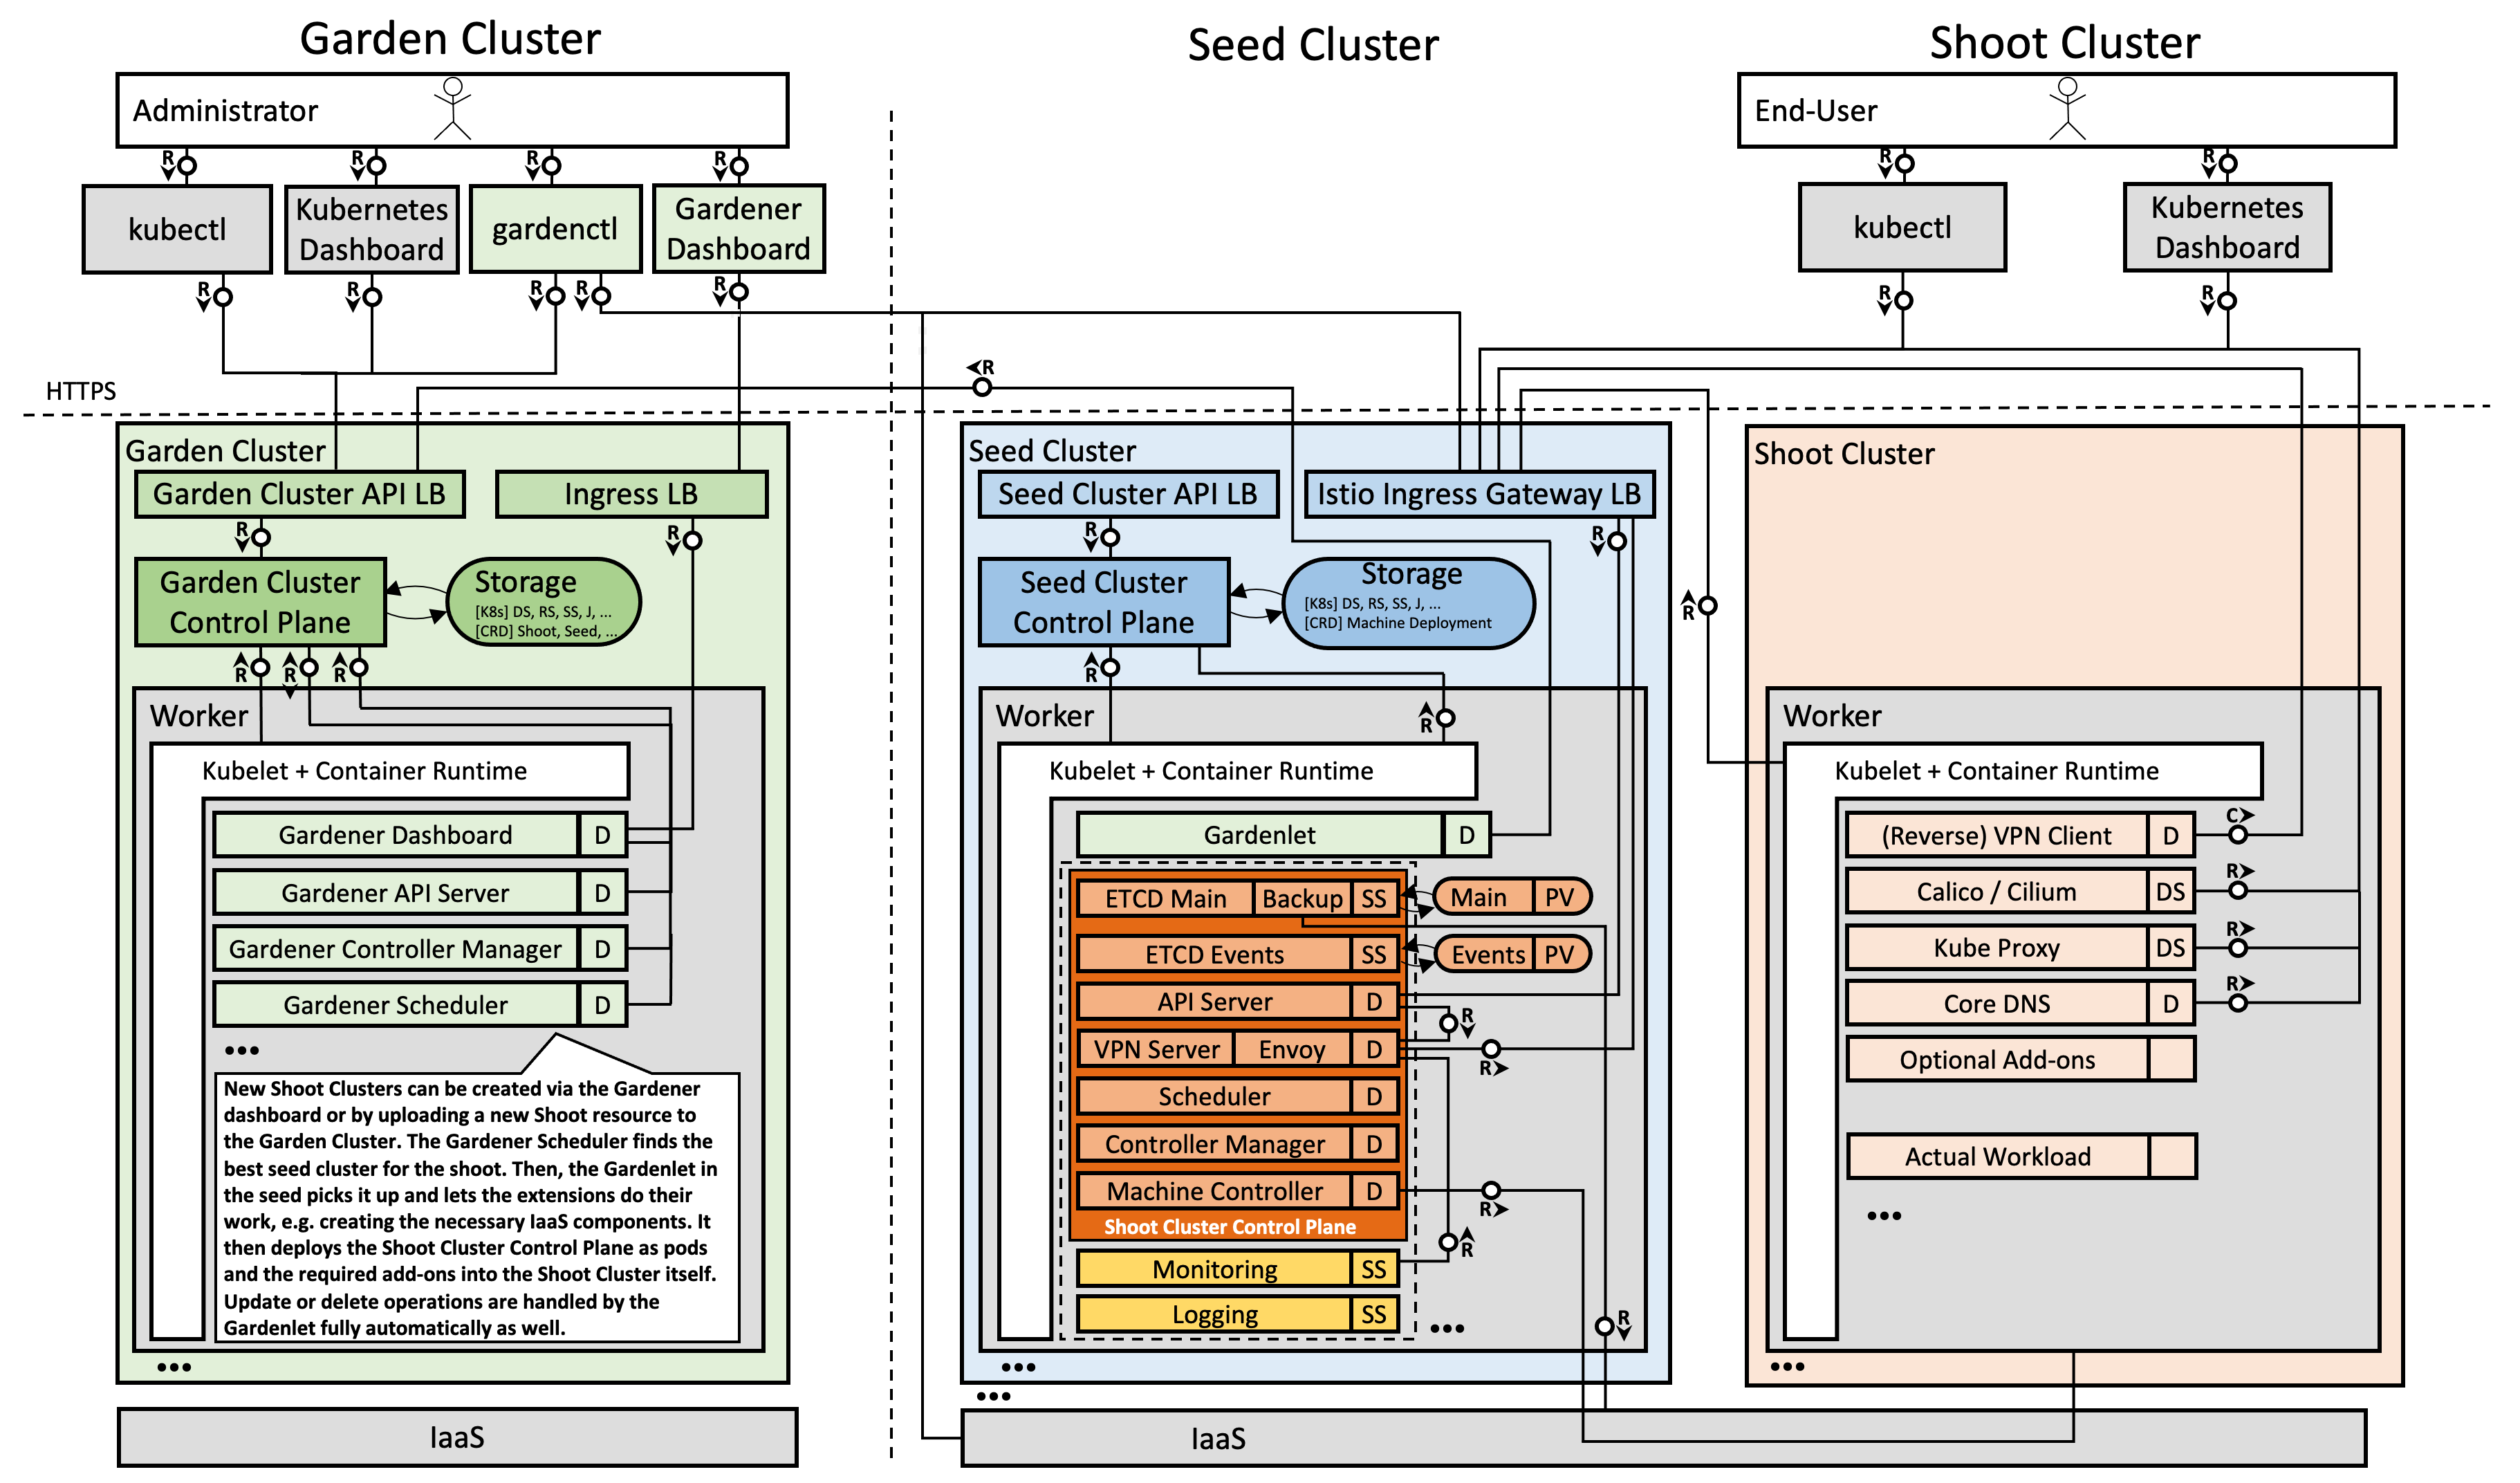
\includegraphics[width=\textwidth]{Bilder/gardener-architecture-detailed.png}
    \caption{Gardener architecture \cite{gardener.architecture}}
    \label{fig:gardener-architecture}
\end{figure}

% \begin{itemize}
%     \item open source software by SAP
%     \item for managing Kubernetes cluster (Kubernetes as a service)
%     \item Kubernetes native extension
    
%     \item cite https://kubernetes.io/blog/2018/05/17/gardener/
%     \item Even though there are tools that help with creating and updating single Kubernetes clusters, it is rather hard to manage many clusters.
%     \item there are tools to help in creating and updating single Kubernetes clusters
%     \item but very hard to manage many clusters
%     \item this is the focus of Gardener
%     \item manages Kubernetes clusters as a service
%     \item Gardener creates Kubernetes-conformant clusters
%     \item supports deployment to multiple cloud providers
%     \item brings the ability to manage thousands of clusters
%     \item 
% \end{itemize}

\section{\ac{aws}}
\acf{aws} is a subsidiary company of Amazon that offers a cloud computing platform with various services, such as \ac{s3} \cite{aws.s3} or \ac{eks} \cite{aws.eks}.
Started in 2006, \ac{aws} nowadays runs data centers all over the world to provide scalable, reliable, and high performing services. \cite{aws.linkedin, whatisaws}

At the time of writing, \ac{aws} is the cloud provider with the biggest market share. \cite{aws.marketshare}
Also, most of the supervising department's cloud service offerings are currently being deployed on \ac{aws}.
Because of these reasons and also due to constraints in time and complexity, the bootstrapping process worked out in this report is going to be narrowed down to deployment in an \ac{aws} environment.

\section{Terraform}
Modern enterprise infrastructure for software development usually makes use of cloud computing to dynamically adapt infrastructure to the fast-paced world of agile development.
These cloud services are usually distributed between multiple infrastructure providers, each of which uses their own individual \acp{api} to configure their platform.
Terraform is a tool that tries to minimize the effort needed to deploy these infrastructures in the long run by automating resource management as far as possible.
It allows to uniformly describe the target infrastructure in an easy to learn, machine-readable definition language and automatically takes care of deploying this infrastructure at the individual \ac{iaas} providers.
This approach is also known as \ac{iac}.
With Terraform, it is also possible to save provisioned infrastructure setups as a Terraform configuration to reuse them at a later point in time or to arbitrarily extend and adapt the configuration.
For configuration, either \ac{json} or \ac{hcl} can be used, with \ac{hcl} being the preferred way by the developing company HashiCorp because of its advanced features compared to \ac{json}.
Terraform can only unleash its full potential because of cooperations with all major software and hardware vendors and providers.
HashiCorp partners with over 160 companies and services the most noticeable ones being:
\begin{itemize}
    \item \ac{aws},
    \item Atlassian,
    \item Cloudflare,
    \item Google,
    \item Microsoft, and
    \item Oracle.
\end{itemize}

The most common use cases for Terraform include general \ac{iac}, managing Kubernetes (\autoref{sec:kubernetes}), multi-cloud deployment, management of network infrastructures, and management of virtual machine images.
Terraform additionally integrates tightly with other HashiCorp services like Vault (\autoref{sec:vault}).

% \begin{itemize}
%     \item codifies cloud apis into declarative configuration files
    
%     \item minimiert langfristig den für das Deploment benötigten Aufwand
%     \item um den modernen Ansprüchen der Schnelllebigkeit gerecht werden zu können, müssen IT-Administratoren Ressourcenmanagement weitmöglichst automatisieren
%     \item Kluster mit maschienenlesbaren Konfigurationscode beschreiben -> Infrastructure as Code
%     \item Terraform ermöglicht einheitliche Beschreibung von Zielinfrastruktur und sorgt für Umsetzung bei IaaS-Providern
%     \item erlaubt es, provisionierte Infrastruktur-Setups zu speichern, um diese zu einem späteren Zeitpunkt erneut nutzen oder beliebig erweitern/anpassen zu können
%     \item 160 Partner, sind unter anderem AWS, Atlassian, Cloudflare, Google, Microsoft und Oracle
    
%     \item üblicherweise wird auf verschiedene Cloud-Services zurückgegriffen um Infrastruktur für die Software-Entwicklung zu realisieren
%     \item daher menge verscheidedner Schnittstellen
%     \item mit Terraform aber nicht
%     \item statt individueller schnittstellensprache konfiguration über json oder HashiCorp Configurration Language (HCL)
%     \item hcl erlaubt kommentare und weitere features gegenüber json
    
%     \item Zusammenarbeit mit allen wichtigen Software und Hardware-Providern
    
%     \item häufige Anwendungsfälle für Terraform:
%     \item Infrastructure as Code
%     \item Multi-cloud deployment
%     \item Manage Kubernetes
%     \item Netzwerkinfrastruktur verwalten
%     \item Images von virtuellen Maschinen verwalten
%     \item Integration mit anderen HashiCorp Plattformen wie Vault
    
%     \item cite https://www.ionos.de/digitalguide/server/tools/was-ist-terraform/
%     \item cite https://www.terraform.io/
% \end{itemize}

\section{Jenkins}
Jenkins is a widely used open source automation server build with Java.
It is a \ac{cicd} tool aiming to save time by automating repetitive tasks like building projects, running test sets and deployment.
Jenkins supports many plugins (over 1800) via its update center which give you the ability to integrate with most of the common tools in development and automate practicably any project.
Jenkins can also be deployed on multiple machines to spread load and ensure quick and efficient operation.
\cite{jenkins.io, jenkins.github, gitlab.cicd}

In context of this project, Jenkins will be used after the successful bootstrap to take care of running Terraform and performing the actual deployment.

% \begin{itemize}
%     \item widely used open source automation server
%     \item built with Java
%     \item CICD tool (Continuous Integration and Continuous Delivery)
%     \item save time by automating repetitive tasks
%     \item like building projects, running tests and deployment
%     \item support for many plugins (over 1800) with its update center
%     \item give you the ability to deploy and automate any project
%     \item can be deployed on and spread load across multiple machines
%     \item cite https://www.jenkins.io/
%     \item cite https://github.com/jenkinsci/jenkins
    
%     \item 
% \end{itemize}

\section{Vault}
\label{sec:vault}
Vault is an open source service with the primary task to provide a central control unit to manage and organize enterprise secrets.
It encrypts secrets both at rest and in transit.
Access to the secrets can be granted granular per user through the use of \acp{acl}.
Furthermore, Vault audits access to the secrets.
That means that it keeps a detailed log on whom accessed what secret at which point in time.
If there was a security breach, where an unauthorized person got access to Vault, this protocol can be used to tell, if a specific secret has been read by the attacker or if it is still safe to use.

Vault is designed to be highly pluggable.
An instance is composed of \emph{storage backends}, \emph{audit log instances}, \emph{authentication providers} as well as \emph{secret backends}.
Each of these can be impersonated by a variety of different components.
This makes it possible to use different trusted authorities for attestation of identity.
For example, among others LDAP, JWT, GitHub, and Radius can be used.
An automated build service could very well use a different service to authenticate to Vault than a human user.

Secrets and encryption are often the weak spot in applications.
If a secret gets leaked and the leak stays unnoticed, attackers could gain long term access to a system.
As a solution, Vault offers \emph{dynamic secrets}.
When a client requests the access credentials for a supported system, Vault creates a short-lived secret just for that specific client.
Because the client is only accessing Vault, it does not have to bother with key creation nor rotation and an increased layer of security is added by not using secrets for an extended period of time.
Also, if a dynamic secret gets leaked, this single secret can be revoked individually.
If all clients accessing the resource used the same credentials, changing or blocking those could potentially cause an outage of the whole system.

When it comes to encryption, it can happen rather quickly that a single mistake compromises the security of the whole application.
Because of this, Vault offers encryption as a service.
The idea is, that Vault concentrates on the single task to handle credentials and encryption safely.
The broad variety of applications have a different focus and are not developed with the necessary expertise to guarantee safe implementation of security measures.
Vault, on the other hand, uses implementations that are audited by the open source community as well as independent experts.
Those are then provided as a high level \ac{api} to application developers.
That way, the encryption process of data gets very easy while, at the same time, Vault can handle the used encryption keys directly, and they are never actually sent to the application itself. \cite{vaultproject.io}

During the bootstrap, this project is about, a technical user is created for Terraform operations.
An access key is created for this user and then saved to Vault.
This way Jenkins then can obtain this access key and use it to perform the actual deployment with Terraform.

% \begin{itemize}
%     \item manage and organize secrets
%     \item provide a central secret storage
%     \item encrypt secrets at rest and in transit
%     \item ACL
%     \item Audit; log who has access what and when
%     \item a secret is a set of different credentials
%     \item protect sensitive data
%     \item various authentication methods; like LDAP, JWT, GitHub, Radius
%     \item authenticate against trusted sources of identity
%     \item trusted authority for attestation of identity
%     \item automate key issuance and rotation
    
%     \item dynamic secrets
%     \item create secrets for each specific client with limited lifetime
%     \item revoke a specific secret targeted
    
%     \item encrypt as a service
%     \item named key
%     \item high level API to do cryptography (encrypt, sign, verify, ...)
%     \item key and encryption logic never actually gets to the developer
%     \item control key lifecycle safely
%     \item protect application data at rest
    
%     \item highly pluggable
%     \item storage backends
%     \item Audit log instances
%     \item auth
%     \item secret backends (key/value, DB plugins, AWS, ...)
%     \item all of these are modular and can use solutions of various providers
    
%     \item cite https://www.vaultproject.io/
% \end{itemize}

\chapter{Conceptional Thoughts}
\label{sec:concept}

\section{Interaction with Services}
Before implementing the bootstrap, one of the major questions is what way should be chosen for programmatically interacting with the services \ac{aws} and Vault.
Both provide multiple possibilities.

\subsection{\ac{aws}}
When it comes to \ac{aws}, there are three obvious ways that could be chosen.

\paragraph{\acs{rest} \ac{api}}
Practically all required \ac{aws} functions can be accessed via its \ac{http} \ac{api}.
Since Go's standard library natively includes a \ac{http} client, utilizing this would be a very lightweight solution.
You would just have to instantiate a \ac{http} client object in Go.
This object then already has all the required functionality to send requests to the \ac{api}.
An \ac{api} call is made through a \ac{http} request with a specific method (GET, POST, PUT, DELETE etc.) to an \ac{api} endpoint.
This endpoint is specific to the operation you want to perform and represented by an \ac{url}.
Additional parameters and input data for the operation can be specified in a key value style via \ac{url} parameters, the request header, or the request body.
\ac{url} parameters can be generated with string replacement and then appended to the base \ac{url} for the \ac{aws} \ac{api}.
The request body is a bit more complex to construct.
It is basically a structure, that maps strings to basic data types or subordinate maps.
This has to be constructed as a structure within Go and can then be encoded into a format supported by the \ac{http} client.

Generally, using the \ac{http} \ac{api} would grant great flexibility because you construct all the requests on your own and therefore have detailed control over what happens without any additional layer of abstraction.
On the other hand, since multiple different \ac{api} calls are required, every single one of the needed calls would have to be manually constructed.
This is a lot of work, prune to errors that are hard to debug, and has a bad influence on the readability of the code in general because the \ac{api} calls would get prevalent to the actual program logic.

\paragraph{\ac{aws} \ac{cli}}
The \ac{aws} \ac{cli} provides a very easy and intuitive interface to the user for interacting with \ac{aws}.
Theoretically, it is intended to be explicitly installed on a system and to be used by a human user rather than programmatically.
Anyway, Go natively provides the functionality to execute commands on system level.
By this mean, also the \ac{aws} \ac{cli} could be used in the program.

But using the \ac{cli} would imply multiple drawbacks.
\acp{cli} often do not have a stable human interface and therefore the output returned by the \ac{cli} is subject to change.
This is no good if the program has to parse the output and behave according to the results because the program could break easily and unnoticed just by updating the \ac{cli}.
Although, in the special case of the \ac{aws} \ac{cli} the user can choose between several output formats including \ac{json} notation, so a changing interface probably would not be of a problem.
What is more of a concern is the fact that the \ac{cli} containing the bootstrap should be part of a container image packing various tools to work with clusters.
The \ac{aws} \ac{cli} is entirely written in Python.
If the \ac{aws} \ac{cli} should be used, Python would have to be installed into this container as well noticeably increasing the resulting image size.
Also, when run locally, the Go application would have to rely on an existing installation of the \ac{aws} \ac{cli} to function correctly or check for its existence and prompt the user to satisfy the dependency manually in case it is missing.
Just running the Go application executable would not be sufficient to perform the bootstrap.
Because of these reasons, embedding the \ac{aws} \ac{cli} into the newly created Go \ac{cli} coordinating the bootstrap should be seen as a solution of last resort.

\paragraph{\ac{aws} Go \acs*{sdk}}
The \ac{aws} \ac{sdk} is a library provided by Amazon itself to interface its \ac{aws} services.
It is not only available for Go but for a variety of different languages.
To make use of it, during development it can be acquired with \code{go get} and imported into the program.
In doing so, you specifically select the needed submodules minimizing the overhead.
Then, the \ac{sdk}'s functions can be normally used inside the Go program.

One notable pain point is the partly ambiguous documentation, dependent on the part and version of the \ac{sdk}.
For instance, while the methods for user management have well documented error codes in version 1 of the \ac{sdk}, telling you exactly what kind of errors you can expect, while version 2 -- which supposedly does a better job on error handling -- does not bother to take note on the possible error types, sometimes requiring in depth research to discover what you can expect.
Luckily, errors are not of a big concern for this project, as near to all kinds of occurring errors just mean an unrecoverable program state and cannot explicitly be handled by the application itself.
Furthermore, \acp{sdk} bring the inherent problem, that you completely rely on the provider in terms of update.
If \ac{aws} changed their \ac{api} while not touching the \ac{sdk}, the program would stop working with no way to fix it rather than waiting for Amazon to update the rest of their codebase.
On the other hand, since this is not a third party but an official \ac{sdk}, one could also see an advantage in it.
Staying with the example of the changed \ac{api} and assuming that the \ac{sdk} gets updated at the same time as the \ac{api}, our codebase would simply continue to work.
At the same time, you would be responsible to update a program utilizing the \acs{rest} \ac{api} entirely on your own.
As, in this case, the \ac{sdk} is released and maintained by Amazon their selves, and because of the introduced simplicity of working with an \ac{sdk} rather than the \ac{api} directly, this variant will be used in the following.

\subsection{Vault}
The aspects and options to consider for Vault are very similar to those for \ac{aws}.
Vault also has an \ac{http} api, a \ac{cli} and an own Go \ac{sdk}.
One noticeable difference here is that -- even though the \ac{sdk} is provided by the vendor itself -- the documentation for the \ac{sdk} is not good at all, especially in terms of login.
To get some login methods running, one has to dig rather deep.
Some functionality simply is not documented at all.

But the by far more important points are, that the newly created \ac{cli} by the supervising department already contains some work in progress parts that interact with Vault.
It would not make much sense to reimplement key aspects that these solutions already cover.
Furthermore, mixing different approaches to access Vault would be bad practice as it makes things unnecessarily complex and introduced multiple points of failure for key functionality.
Because of this, Vault's \ac{http} \ac{api} will be used in this project.
This can be additionally reasoned with the advantages of \ac{http} \acp{api} described in the predeceasing section with the difference, that there are not many functions of Vault that need to be accessed despite reading and writing secrets.
The programming overhead in writing these interactions manually via the \ac{http} client is pretty small.

\section{Assumptions}
The before mentioned container image already contains scripts to manage login to \ac{aws}.
These scripts take a \ac{saml} response and generate the file \code{\textasciitilde/.aws/credentials} out of it.
This file contains sets of \ac{aws} credentials consisting of an access key ID, a session token and a secret key.
These credential sets are sufficient authentication information to interface \ac{aws}.
For the following implementation, the assumption is made, that this file already exists and contains a valid key set.

\section{Policy Management}
In \ac{aws} a policy grants access to specified resources like \ac{s3} storage buckets.
During the bootstrap, a technical service user is created for Terraform which needs the rights to access the Terraform state bucket.
To grant these permissions, a policy is needed.
There are different types of policy that can be chosen from, the two most noticeable ones being \emph{managed policies} and \emph{inline user policies}.
A managed policy is an own entity that is created and can exist independently of a user or similar objects.
To grant a user the rights that the policy grants, the policy is \emph{attached} to the user.
An inline policy on the other hand is a property of the user it is attached to.
In does only apply to this single user and cannot be attached to different users, groups or roles.

The policy created in the bootstrap will only be used for the terraform user.
Therefore, theoretically it would be the proper way to go to use an inline policy so that the list of other policies does not get cluttered unnecessarily.
Although, different size limits apply to the different policy types.
The total size of all inline policies that can be attached to a user must not exceed 2048 bytes.
Because the cluster name is used multiple times in the policy, if you do the calculation, it becomes clear that the usage of inline policies would entail harsh length limits on the cluster name that would not be reasonable.
Therefore, managed policies will be used even though the management has a bigger overhead.
\chapter{Implementation}
As the supervising department already works on the \ac{cli} in which the bootstrap shall be included, the following implementation will take part inside an existing Go project.

Go programs are structured into packages that logically separate different aspects and functionalities.
Most of the development in this section is directly connected to interfacing with \ac{aws} and will therefore take place inside the newly created \code{aws} package.

The bootstrapping process will have to traverse the following steps in order:
\begin{enumerate}
    \item create an \ac{s3} bucket as a state storage for Terraform
    \item create Terraforms technical user
    \item create or update the access policy for the technical user
    \item attach the access policy to the technical user
    \item if access keys exist, check them for expiration
    \item if keys are expired or do not exist, perform a key rotation
    \item safe newly generated keys to Vault
\end{enumerate}
As this process is too long and complex to present it in all its details, excerpts will be used to exemplarily present the process of formation.

\section{AWS Client Struct}
A struct in Go is basically a collection of named values that forms a new type.
This is used to group data together and can be somewhat compared to objects in other programming languages.
Functions can be bounded to a struct type, forming methods that can perform operations on the contained data.

This principle will be used to build a custom \ac{aws} struct for performing the bootstrap.
The result can be seen in \autoref{code:aws-struct-1}.
On the one hand, the struct stores a general configuration and access clients to the needed \ac{aws} services (lines 2-5).
The configuration, for example, contains the information on which global region the operation should be performed (like \code{us-east-1} or \code{eu-central-1}).
The access clients are for \ac{s3}, \ac{iam}, and \ac{sts}.
The types of these fields are defined by their respective \ac{sdk} packages.
The following variables are strings needed multiple times across the different operations.

\lstinputlisting[
    language = Golang,
    firstline = 29,
    lastline = 41,
    caption = \ac{aws} struct (excerpt from aws.go),
    label = code:aws-struct-1
]{Quellcode/base/aws.go}

All the variables are not meant to be set by hand but through a constructor.
The constructor (\autoref{code:aws-constructor-1}) takes the desired region and cluster name as input parameters and ensures that the other values get set properly.
First, a configuration is loaded from default values (lines 4-9).
In this step, also the afore-mentioned credentials get loaded into the configuration.
The constructor also packs the ability to return errors.
For instance, errors could occur when loading the configuration (line 4).
If this is the case, \code{err} would be something different from \code{nil} (line 5), the error gets logged (line 6) and returned alongside a nil value for the \ac{aws} struct (line 7) because obviously a successful generation was not possible.
After loading the configuration, the region is set and the other names are generated based on the given cluster name and region (lines 11-17).
In lines 19-21, new clients are constructed for \ac{s3}, \ac{iam}, \ac{sts} and persisted in the struct.

The \ac{aws} account ID is for instance required to generate \acp{arn}.
In this project, \acp{arn} are needed to access policies.
Therefore, the account ID needs to be obtained.
The \ac{sdk}'s \ac{sts} client has a method to get details on the identity of the calling user and returns a struct which also contains the account ID.
First, the identity struct is loaded (lines 24-28) then the ID is extracted and saved to the \ac{aws} struct.
As the \ac{arn} of a resource can be clearly calculated with the account ID, the resource type, and the resource name, the \ac{arn} for the policy can already be calculated and saved to the struct (line 30).
The constructor then returns the finished struct.

\lstinputlisting[
    language=Golang,
    firstline = 43,
    lastline = 76,
    caption = Constructor for the \ac{aws} Struct (excerpt from aws.go),
    label = code:aws-constructor-1
]{Quellcode/base/aws.go}

\section{Checking \ac{aws} State and Creating Objects}
The aim of this bootstrap is, that all necessary objects, users, and access rights exist in \ac{aws}.
Although, it is unclear, which of these might already exist.
So for each of those entities, one has to check whether they exist and create them if they do not.
As the process for each of these is quite similar, it would go beyond the constraints of this report to explain each of the steps in detail.
Instead, this process will be explained by the means of creating the \ac{s3} storage bucket for Terraform.

As briefly outlined above, the first action must be to check whether the bucket already exists as the bucket should not be overwritten if it already existed.
This is done with the \ac{sdk} method \code{HeadBucket} (lines 2-3) which receives the desired bucket name as input.
The method call returns an output and an error.
For checking bucket existence, only the error is relevant and saved to the variable \code{err}.
The output can be discarded and therefore only an underscore is written instead of a variable name.

The \ac{sdk} wraps all service errors as \emph{\ac{api} errors}.
To check, if and what error occurred, the error is interpreted as \code{smithy.APIError} (lines 6-8).
After this, it can be checked against the error types defined by the \ac{s3} \ac{sdk} package (line 9).
The relevant error type is \code{NotFound}.
If this error is on hand, the bucket does not exist and has to be created (lines 11-22).

Creating an \ac{s3} bucket via the \ac{sdk} is pretty simple but has a little trick to it.
The default \ac{aws} location to create buckets in is \emph{us-east-1}.
If and only if a bucket shall be created in a different location, one has to specify a so-called \emph{LocationConstraint}.
Because of this, the configured region is checked to select the correct \ac{sdk} method call accordingly.
If creating the bucket is free of errors, the method returns nil at this point, otherwise the creation error is returned (lines 24-28).
If no error occurred in the first place, then this means a successful call of the \emph{HeadBucket} method and therefore it means that the specified bucket exists.
In this case, nothing happens and the method returns nil (line 33).

\lstinputlisting[
    language=Golang,
    firstline = 78,
    lastline = 111,
    caption = Creating the Terraform State Bucket (excerpt from aws.go),
    label = code:aws-bucket-creation
]{Quellcode/base/aws.go}

\section{Policy Generation from File}
In \autoref{sec:concept} the difference between managed and inline policies, and also why managed policies will be used, was already covered.
To create a policy in \ac{aws}, an \ac{sdk} method, similar to the one applied in the predeceasing section for creating the \ac{s3} bucket, can be used.
But to do so, a so-called \emph{policy document} needs to be passed to the method.
This is basically a \ac{json} string in which the access to the desired resources is specified.
In case of this bootstrap, the policy document will need to contain the specific names of the needed \ac{s3} buckets.
As these names are dependent on the specified cluster name, the \ac{json} string needs to be build accordingly.
To accomplish this, Go's standard library packs a functionality called \emph{templates}.
A template in Go is a string containing special symbols to mark the positions in the text that shall be replaced.
These symbols are generally indicated by double curly braces.
The braces then contain a key indicating with what property they should be replaced.
In the given case, just one string needs to be replaced at multiple places in the entire time.
Therefore, only the symbol \code{\{\{.\}\}} is needed.
The beginning of the policy file can be seen in \autoref{code:policy.tpl}.

\lstinputlisting[
    firstline = 1,
    lastline = 9,
    caption = Template File for the \ac{aws} Policy (excerpt),
    label = code:policy.tpl
]{Quellcode/base/terraform_policy.tpl}

But the let alone existence of this template file is not sufficient to make use of it.
A new method (\autoref{code:aws-policy-generation}) is written, to wrap the needed method calls of Go's template package to parse the template and build the actual policy from it.
First, the template string is loaded, that in this case resides in a separate file.
This gives the opportunity to change the template later on without recompiling the code.
This saves time and effort, and also, it might not even be possible to recompile because the source code is only available internally.
Files can be read in Go with the use of the \code{iotuil} package from the default library.
When calling the \code{ReadFile} method, the path to the file has to be given as a string and a byte slice is returned (lines 2-6).
Then, a new template can be parsed from the slice (lines 7-11).
During the parsing process, the template package checks for syntax errors in the template file and aborts execution if errors occur.
Finally, the policy gets \emph{executed}.
To do so, the string that should substitute the placeholders and a bytes buffer has to be passed to the templates \code{Execute} method (lines 13-17).
This buffer can then be converted to a string and is returned by the method (line 18).
The returned result is now ready to be used as a policy document.

\lstinputlisting[
    language=Golang,
    firstline = 164,
    lastline = 182,
    caption = Method for Policy Generation (excerpt from aws.go),
    label = code:aws-policy-generation
]{Quellcode/base/aws.go}


\section{Key Rotation}
Another important aspect in cloud computing, especially in the matter of long-term maintenance, is access key management.
Of course, it is very important to use secure keys and keep them secret.
But frequently renewal of keys may not be neglected.
That way, even if an attacker gains access to a key, this will not be a problem for long.
Although, this may sound simple, it has to be taken care that no legitimate user gets locked out of the systems during this process.
\ac{aws} therefore supports the parallel management of two access keys.
That way, a key can be deleted and renewed while, in the meantime, access to the system remains undisturbed with the other key.
This process is called \emph{key rotation}.

The bootstrapping procedure shall perform a key rotation if keys already exist for the technical user and a key exceeds a maximum age of seven days.
The age of a key can be determined by its metadata.
\autoref{code:aws-key-rotation} shows how the check is performed on whether a new key has to be created or not.
The method takes a slice of access keys to check as parameter and returns a boolean that indicates if a new key has to be created in the following (line 1).
Since an \ac{aws} user can have anything between none and two access keys, there are three different cases to be distinguished.
The first and most basic case is when no access keys exist for a user.
In this case the length of the input slice is zero and a new key has to be created (lines 2-5).

If the Terraform user has exactly one access key, there are two possibilities.
Either the key is younger than seven days and nothing happens or the key exceeds the maximum age of seven days and a new key has to be created (lines 7-14).
The key is not deleted in this case because if this would be the very key that is currently being used for automated access through Jenkins, this would block the service out.
Instead, deleting the old key will happen the next time the bootstrapping procedure is executed.
This way, there is no danger of accidentally blocking the access of a service.

If two keys exist, the older one of the two has to be determined first.
Since it is known that there never ever will be more than two keys and the cases for zero keys and one key is already handled, it can safely be assumed that the first and second index of the input slice contains valid access keys.
Therefore, it is very easy to determine the oldest key with a simple if statement (lines 16-19).
After this, the procedure is very similar to the case with only one access key.
It is checked, if the key is older than seven days (line 20).
If this is the case, a new one has to be created (lines 29-30), although this time the old key gets deleted (lines 21-28).
If the key is younger than these seven days, again nothing happens (lines 33-34).

\lstinputlisting[
    language=Golang,
    firstline = 325,
    lastline = 359,
    caption = Key Rotation (excerpt from aws.go),
    label = code:aws-key-rotation
]{Quellcode/base/aws.go}

\section{Updating Keys in Vault}
Every time a new key gets created, it needs to be saved to Vault.
As already mentioned in \autoref{sec:concept}, there is already an implementation of a basic Vault client by the supervising department that just needs to be extended to add the functionality to add keys to Vault.
For this purpose, the method shown in \autoref{code:vault-update} is added to the existing Vault package.

The method binds to a config struct that satisfies a Vault client interface, stores information like the vault address and the path where the secret shall be created or where it can be accessed.
The access key to be saved is passed to the function as a parameter (line 1).
Then, the call to the Vault \ac{api} is prepared.
First, the endpoint \ac{url} is constructed from the Vault base address and the desired secret path (line 2).
Then, the request body containing the new secret is prepared.
Vault takes new secrets from the \emph{data} sections of \ac{json} bodies.
Therefore, a new map is created and the passed access key is mapped to the key \code{data}.
Go then provides a method, again from its default library, to convert an ambiguous map into a \ac{json} bytes slice (lines 4-6).
Then, a new \ac{http} client is constructed (line 8).
Also, a new \ac{http} request gets build.
The request will be of type \code{POST}, targeted to the determined \ac{url}, and utilizing the generated \ac{json} body (line 9).
The header of the request must contain a Vault token for authentication.
This token is already available in the config struct and can simply be added to the request header (line 10).
The \ac{http} client is then used to send the request (lines 11-15).

\lstinputlisting[
    language = Golang,
    firstline = 252,
    lastline = 267,
    caption = Saving Keys to Vault,
    label = code:vault-update
]{Quellcode/vault.go}

\chapter{Future Work}
To finish off the bootstrap, work beyond the scope of this report is required.
Some fundamentals and considerations regarding these tasks shall be discussed here, although their realization will not be depicted.

\section{Establishing Tests for the Bootstrap}
When it comes to testing the implemented solution, it is important to distinguish different categories of tests.
On the one hand there are \emph{unit tests} and on the other there are \emph{integration tests}.

\paragraph{Unit tests} are about testing small components of code for functionality in different scenarios.
Do to so, the test often isolates the components from the remaining code.
Dependencies on other systems are usually swapped out to create this isolation.
This process is called \emph{mocking}.
In general, unit tests should not have side effects and should be completely independent of the rest of the application.
Because of this, unit tests are very fast, simpler in structure and therefore also easier to write.

\paragraph{Integration tests} on the other hand are way more complex than unit tests.
Like their name suggests, they test the integration of a module with other modules.
This is done when a unit test is not sufficient for testing some functions because of its isolation property.
Integration test do not try to mitigate side effects but consider them from the beginning.
Generally, integration tests are more complex to set up and slower than unit tests.
Also, integration test might often rely on external resources which failures are beyond the control of the developer.
As a result, it is usually desirable to use many unit tests and only few integration tests.

The difficulty with the implementation of the bootstrap at this state is that the interaction with \ac{aws} is deeply tied into the business logic of the bootstrap.
As a result, the bootstrap would require integration testing as a verification, although an integration test should only cover the actual interaction with \ac{aws} and not the bootstrap itself which should rather be checked with basic unit tests.
To cover the business logic of the bootstrap with unit tests, the bootstrap therefore has to be decoupled from the interaction with \ac{aws}.
The \ac{aws} part would then have to be covered with an integration test, although a much smaller one, which could focus solely on the third party service and would not get mixed with the departments own business logic.
To do so, there are different approaches that can be chosen from.

\paragraph{Client Interfaces} A common approach to write unit tests for something like the bootstrap would be to replace the clients of the \ac{aws} \ac{sdk} that communicate with the \ac{aws} backend with mocked clients.
These mocked clients could then fake the interaction with \ac{aws} and deliver reproducible results to test the actual business logic.
In Go, this is generally rather easy to achieve through the use of interfaces.
An interface in Go is just a definition of method headers.
Any type that implements the specified methods, automatically also implements the interface.
For making the actual clients interchangeable with mocked clients, interfaces would have to be specified, that define all \ac{sdk} methods the clients need.
Then, new types could be constructed, that implement those methods and return the desired values for mocking.
Now, instead of using the types of the actual \ac{sdk} clients when referring to the clients (in this case the types of the client variables in \autoref{code:aws-struct-1}), the interfaces would be used.
This enables the tests to replace the clients with the mocked clients without changing the program execution, because the same methods can be called but just on different objects.

This is an easy approach if only a few methods have to be mocked.
The problem in the context of this project is, that especially for the \ac{iam} client, many methods would have to be mocked individually, which is a lot of work, creates a lot of overhead for creating the interface, and it is difficult to cover all special cases and possible errors.

\paragraph{Function Pointers}
In some ways, this approach is rather similar to the aforementioned one.
In Go, functions can be stored in variables just like anything else.
So by extracting certain functionality into individual functions, instead of creating entire mock clients, just some functions could be swapped out for other functions delivering the mocked results.
To make use of this principle, another layer of abstraction would need to be implemented that wraps the \ac{sdk} methods into package scoped functions, and, if feasible, aggregates multiple \ac{sdk} methods into one wrapper.
These wrappers could be referred to with function pointers.
For unit testing, only these pointers would have to be adjusted to point to the mocked methods.
This can happen directly in the test file as in Go the tests are located in the same package.
The wrappers themselves could be verified for functionality with integration tests.

Although this approach reduces the complexity of the actual mocking by omitting the use of interfaces and rebuilding the entire clients, as a downside it would require some restructuring to the code because the calls to the \ac{sdk} methods would have to be replaced with the function pointers.

% \section{Integration with the \ac{cli}}
\chapter{Evaluation}
In the course of this project, a working prototype of the bootstrapping process required for automated deployment of cloud service offerings via Terraform was successfully implemented in an existing Go project.
The scope was momentarily restricted to support \ac{aws} only.
It was discussed what means should be chosen for interacting with third party services.
The official \ac{aws} Go \ac{sdk} and the Vault \ac{http} \ac{api} were found to be the appropriate choices in the context of this project.
Different ways of policy management for \ac{aws} were compared and classified in terms of their suitability.
The functionality for the bootstrap was then implemented in a dedicated Go package.
The implementation of the package reached a state where the bootstrap is functional and could technically be included in the actual \ac{cli}, although automated testing still have to be established until it can be considered final.
Two different approaches for testing were discussed.
Since a restructuring of the code is likely to be necessary for the realization of these tests, the solution was not yet integrated into the \ac{cli} for the time being.

Even though the solution is not yet included in the actual \ac{cli}, for the most part, the defined goal can be considered achieved.
As the bootstrap package does not handle user authentication on its own, no user interaction is required for performing the bootstrap despite the initial call to the \ac{cli}.
Thus, the execution environment also does not matter.
Therefore, the bootstrapping process will be usable both by physical users and by automated build servers.
The remaining step to reach the goal is adding the bootstrap as a \ac{cli} command which is rather easy once the actual functionality reached its final state.

Economically, the implemented solution will pay off in the future.
The benefits in terms of time and cost of automating a manual task, consisting of multiple steps, are clear -- especially if this task is executed many times.
The bootstrap itself is part of a much larger deployment process.
In complex processes, the sum of individual improvements quickly adds up.
Also, by not relying on external scripts to automatically perform the bootstrap but integrating the functionality directly into the very \ac{cli} that is used for other tasks related to SAP's cloud service offerings, the footprint of necessary tools is reduced.



% Goal of this project is to simplify the bootstrap by integrating the necessary functionality into a \acf{cli} which is currently developed by the supervising department.
% Also, the usage should be convenient and, beside providing login data for the cloud provider and credential store, minimal user input should be required to perform the bootstrap.
% Furthermore, the newly developed \ac{cli} is required to be able to get executed by an automated build server.
% The ways of user interaction have to be designed accordingly.


% ---- Literaturverzeichnis
\cleardoublepage
\renewcommand*{\chapterpagestyle}{plain}
\pagestyle{plain}
\pagenumbering{Roman}                   % Römische Seitenzahlen
\setcounter{page}{\numexpr\value{savepage}+1}
\printbibliography[title=Literaturverzeichnis]

% ---- Anhang
\appendix
\include{Inhalt/04_Inhalt/1100_appendix}
%\clearpage
%\pagenumbering{Roman}  % römische Seitenzahlen für Anhang

\newpage
\end{document}
